\chapter{Introduzione}

Prima di poter parlare di \textbf{Algoritmi Crittografici \textit{Post Quantum}}, è necessario andare a capire per quale motivo si sono resi necessari.

Il \textbf{\textit{Quantum Computing}} è stato ideato da Yuri Manin e Richard Feynman, che presupponeva di utilizzare i fenomi della \textbf{meccanica quantistica} come la \textbf{\textit{superposition}}, \textbf{\textit{interference}} e \textbf{\textit{entanglement}} per eseguire operazioni sui dati.
\begin{itemize}[nosep]
    \item un \textbf{qubit} è l'analogo quantistico del classico bit, e può essere due valori contemporaneamente con una probabilità diversa per ognuno.
    \item un \textbf{\textit{n-qubit register}} può essere in $2^n$ stati nello stesso momento, ognuno, anche in questo caso, con la stessa probabilità.
\end{itemize}
Quando una funzione $f: \{0, 1\}^n \rightarrow \{0, 1\}^n$ è applicato ad un \textit{n-qubit register}, vengono simultaneamente valutati tutti i $2^n$ stati. Nel momento in cui viene \textbf{misurato} il valore di un \textit{n-qubit register}, questo collasserà su uno del $2^n$ possibili valori secondo la sua distribuzione di probabilità sottostante. In linea di massima possiamo definire i computer quantistici come ``\textit{massively parallel machines}''.

\begin{flushleft}
    \textbf{1.} La minaccia dei \textit{Quantum Computer}: \textbf{\textit{Shor's Algorithm}}\cite{shor}. L'intero sistema \textbf{PKI} utilizza alla sua base tre algoritmi:
    \begin{enumerate}[nosep]
        \item \textbf{RSA}: la cui sicurezza è basata sulla difficoltà della fattorizzazione di numeri interi.
        \item \textbf{DH}: la cui sicurezza è basata sulla complessità del \textit{discrete logarithm problem}.
        \item \textbf{ECC}: la cui sicurezza è basata sulla complessità del \textit{elliptic curve discrete logarithm problem}.
    \end{enumerate}
    Nel 1994, Peter Shor ha scoperto un algoritmo quantistico efficente (\textit{polynomial time}) per risolvere questi problemi. In questo modo, tutte le implementazioni RSA, DH e ECC possono completamente risolte dai computer quantistici.
\end{flushleft}

\newpage

\begin{flushleft}
    \textbf{2.} La minaccia dei \textit{Quantum Computer}: \textbf{\textit{Grover}}\cite{grover}.
    \begin{boxA}
        Consideriamo una funzione $F: \{0, 1\}^n \rightarrow \{0, 1\}$ tale che:
        \begin{itemize}[nosep]
            \item $F$ è facilmente calcolabile
            \item $F(x) = 1$ per esattamente un input $x \in \{0, 1\}^n$
        \end{itemize}

        \textcolor{blue}{\textit{Grover's algorithm}}: nel 1996, Lov Grover ha scoperto un algoritmo quantistico che permettesse di trovare la $x \in \{0, 1\}^n \; | \; F(x) = 1$ in $\sqrt{2^n}$ valutazione della funzione $F$.
    \end{boxA}
    \textcolor{blue}{\textit{Exhaustive key search}}: se consideriamo AES con una chiave (\textit{secret key}) lunga $\ell$-bit. Supponiamo di conoscere $t$ ovvero una coppia plaintext-ciphertext $(m_i, c_i)$, dove $t$ è tale che il numero di falsi positivi -- è una chiave $k'$ che permette di risolvere $c_i = \text{AES}_{k'}(m_i)$ con $k' \neq k$  -- sulle chiavi è molto vicino a 0.

    Possiamo definire $F: \{0, 1\}^{\ell} \rightarrow \{0, 1\}$ dove $F(k) = 1 \Leftrightarrow \text{AES}_k(m_i) = c_i \; \forall i \in \{1, t\}$ e $F(k) = 0$ negli altri casi. Allora l'algortimo di Grover può trovare la chiave segreta non in $2^{\ell}$ operazioni classiche, ma in $2^{{\ell}/2}$ \textbf{operazioni quantistiche}.
\end{flushleft}

\begin{flushleft}
    \textbf{Timeline dei Quantum Computer} \newline
    \begin{figure}[h]
        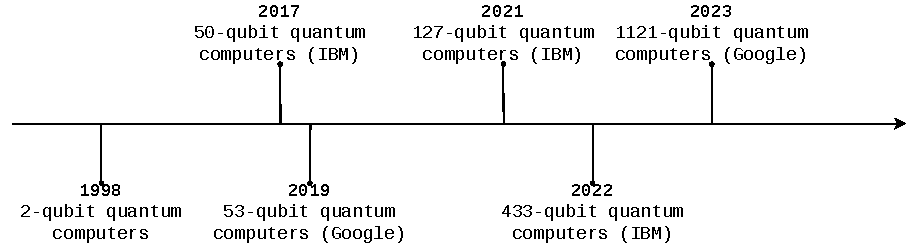
\includegraphics[width=\textwidth]{img/00_quantum_timeline}
        \caption{Evoluzione del numero dei qubits nei Quantum Computer}
        \label{fig:00_quantum_timeline}
    \end{figure}

    Per fattorizzare una chiave RSA a 2048 bit in tempo polinomiale sfruttando l'algoritmo di Shor, un computer quantistico richiede registri composti da diverse migliaia di qubit --- almeno registri a 2048 qubits. Attenzione, però, non tutti i qubit sono uguali: c'è una grande differenza tra \textbf{qubit fisici} (l'hardware reale) e \textbf{qubit logici} (l'unità di calcolo vera e propria). Poiché i qubit fisici sono estremamente delicati e inclini a generare errori per via del rumore ambientale e della decoerenza, non è possibile utilizzarli direttamente per calcoli complessi. Per renderli \textbf{\textit{fault-tolerant}} è necessario applicare il protocollo \textbf{\textit{Quantum Error Correction} (QEC)}\cite{shor_qec}, il quale permette di raggruppare un elevato numero di qubit fisici --- singolarmente instabili e imperfetti --- per sintetizzare un unico qubit logico, stabile e affidabile per il calcolo.

    Viene stimato che siano necessari migliaia di qubit fisici per costruire un qubit logico. In questo modo per riuscire a costruire un registro di almeno 2048 qubit logici sono necessari milioni di qubit fisici. Uno studio del 2021, portato avanti da Gidney e Ekers \cite{Gidney_2021} stima che siano necessari 6,000 qubit logici e 20,000,000 qubit fisici per riuscire a fattorizzare una chiave RSA in 8 ore.

    La minaccia principale, che però non è così immediata, degli algoritmi di Shor e Grover è la possibilità di catturare e memorizzare grosse quantità di traffico internet fino a che non ci sarà la possibilità di decifrarlo senza la conoscenza della chiave privata: \textbf{\textit{Harvest Now Decrypt Later} (HNDL) \textit{attacks}}.
    \begin{table}[h]
    \centering
    \begin{tabular}{llcl}
        \toprule
        \textbf{Nome Algoritmo} & \textbf{Tipologia} & \textbf{KEM o DSA} & \textbf{Standard} \\ 
        \midrule
        \textbf{Kyber} & Lattice-based & KEM & FIPS 203 \\ 
        \textbf{Dilithium} & Lattice-based & DSA & FIPS 204 \\ 
        \textbf{SPHINCS}+ & Hash-based & DSA & FIPS 205 \\ 
        \textbf{Falcon} & Lattice-based & DSA & FIPS 206 (Draft / In arrivo) \\ 
        \textbf{LMS} & Hash-based & DSA & SP 800-208 \\ 
        \textbf{XMSS} & Hash-based & DSA & SP 800-208 \\ 
        \bottomrule
    \end{tabular}
    \caption{Algoritmi crittografici Post-Quantum standardizzati dal NIST.}
    \label{tab:00_nist_pqc}
\end{table}
\end{flushleft}